\documentclass[tikz,border=4pt]{standalone}
\usepackage{amsmath}
\usetikzlibrary{decorations.markings}
\begin{document}
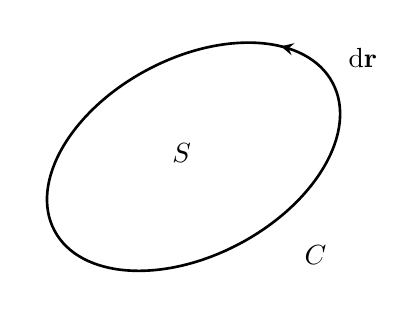
\begin{tikzpicture}[>=stealth, thick, scale=1.0]
  % Closed tilted curve C enclosing region S with counterclockwise arrow dr
  \begin{scope}[rotate=28]
    \draw[line width=0.95pt,
      postaction={decorate},
      decoration={markings, mark=at position 0.08 with {\arrow{>}}}]
      (0, 0) ellipse (2.0 and 1.25);
  \end{scope}

  % Region S inside
  \node at (-0.15, 0.05) {$S$};
  % Curve C label outside bottom right
  \node at (1.55, -1.25) {$C$};
  % dr label near the counterclockwise arrow at upper right
  \node at (2.15, 1.25) {$\mathrm{d}\mathbf{r}$};
\end{tikzpicture}
\end{document}
